Now we will examine what different compression levels might look like.
For this, we will use a sample image to demonstrate its effects.

\begin{figure}[ht]
    \centering
    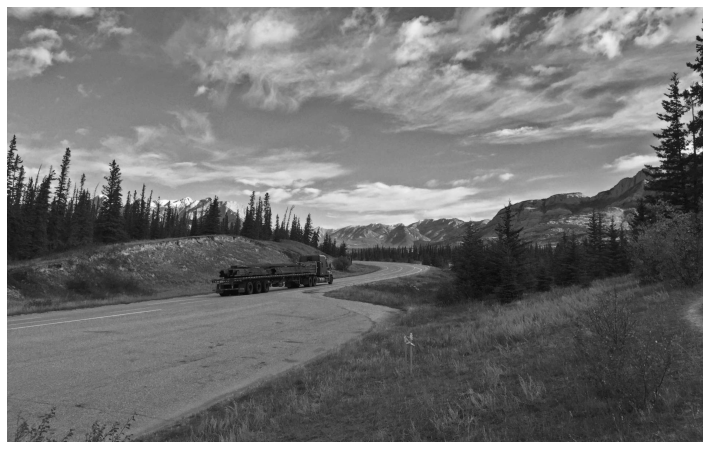
\includegraphics[width=0.725\linewidth]{external_content/media/compression_example/uncompressed.png}
    \captionsetup{justification=centering}
    \caption{Uncompressed image}
    \label{fig:uncompressed}
\end{figure}
\vspace{-2mm}

To begin with, let us consider the uncompressed image in figure \ref{fig:uncompressed} which we will base the compression on.
This image is then translated into an $n \times m$ matrix and decomposed using the \gls{svd}.

After computing the \gls{svd}, we will examine the output when considering various $r$ \acrlongpl{pc} in figure \ref{fig:compressionComparison}.
A compression down to the first 10 \glspl{pc} in figure \ref{fig:compressionNX} shows a considerable decrease in quality.
For this representation we require about 0.8\% of the original data storage.
\medskip

Next up we have chosen the first 50 \glspl{pc} in figure \ref{fig:compressionNL}.
The thumbnail already looks recognisable, meanwhile zooming in does show significant quality downturns.
This compression requires 4\% of the original data size.

Finally, when looking at $r=120$, or 10\% of the original data size, we can still observe some noise in the picture but retain the full level of detail.


% \item Talk about grouping similar areas
% \item Compression example
% \item logplot which shows how much variance is preserved

\begin{figure}[h]
  \centering
  \begin{subfigure}{0.32\textwidth}
      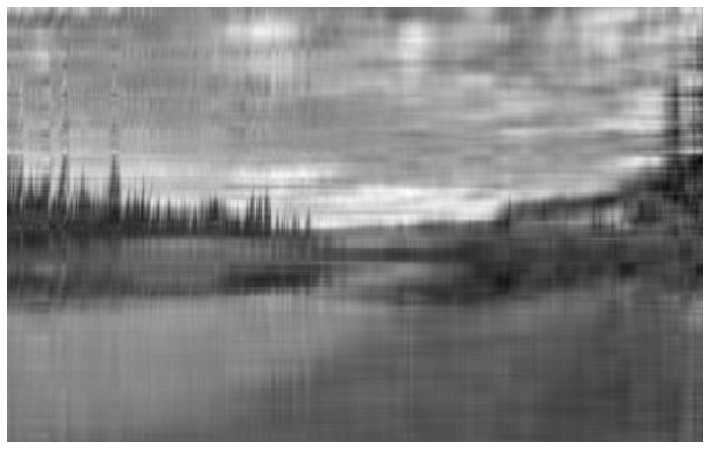
\includegraphics[width=\textwidth]{external_content/media/compression_example/n=10.png}
      \caption{$r$ = 10}
      \label{fig:compressionNX}
  \end{subfigure}
  \hfill
  \begin{subfigure}{0.32\textwidth}
      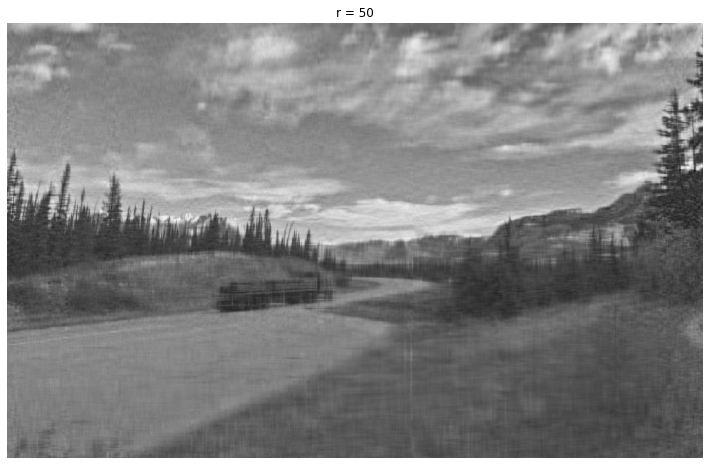
\includegraphics[width=\textwidth]{external_content/media/compression_example/n=50.png}
      \caption{$r$ = 50}
      \label{fig:compressionNL}
  \end{subfigure}
  \hfill
  \begin{subfigure}{0.32\textwidth}
      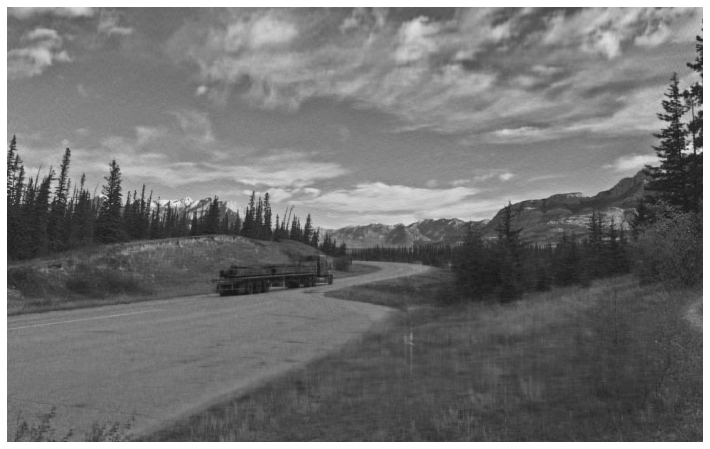
\includegraphics[width=\textwidth]{external_content/media/compression_example/n=120.png}
      \caption{$r$ = 120}
      \label{fig:compressionNC}
  \end{subfigure}
  \caption{Comparison of different compression levels}
  \label{fig:compressionComparison}
\end{figure}
